\documentclass{beamer}

\hypersetup{pdfpagemode=FullScreen} % full screen mode
\setbeamertemplate{navigation symbols}{}

\usepackage[english]{babel}
\usepackage[latin1]{inputenc}
\usepackage{amsmath,amssymb}
\usepackage[T1]{fontenc}
\usepackage{curves}
\usepackage{verbatim}
\usepackage{multimedia}
\usepackage{mathptmx}
\usepackage{graphicx}
\usepackage{booktabs}
\usepackage{hyperref}
\usepackage{multirow}
\usepackage{xcolor}
\usepackage{algorithm,algorithmic}
\renewcommand{\algorithmicrequire}{\textbf{Input:}}
\renewcommand{\algorithmicensure}{\textbf{Output:}}
\usepackage{lipsum}
\setbeamertemplate{caption}[numbered] % for numbering figures

\mode<presentation> {

\usetheme{Singapore}

\usecolortheme{whale}

% \setbeamertemplate{footline} % to remove the footer line in all slides uncomment this line

\setbeamertemplate{navigation symbols}{} % to remove the navigation symbols from the bottom of all slides uncomment this line
}

\usepackage{graphicx}
\usepackage{booktabs}
\setbeamercovered{transparent}
\setbeamertemplate{bibliography item}[text]
\setbeamertemplate{theorems}[numbered]
\setbeamerfont{title}{size=\Large}
\setbeamerfont{date}{size=\tiny}

\setbeamertemplate{itemize items}[ball] % if you want a ball
\setbeamertemplate{itemize subitem}[circle] % if you want a circle
\setbeamertemplate{itemize subsubitem}[triangle] % if you want a triangle

%-------Customized Frame-------
\newcounter{cont}

\makeatletter
\setbeamertemplate{frametitle continuation}{
}
\makeatother

%--------------------------
%	TITLE PAGE
%--------------------------

\title[Project II]{Project II} % the short title appears at the bottom of every slide, the full title is only on the title page

\author[Tang Quoc Thai]{\texorpdfstring{{\normalsize Tang Quoc Thai}}{Author}}

\institute[2270376] % matricola
{

{\small Supervisor}\\
\medskip
{\small Assoc.\ Prof.\ Quan Thanh Tho}\\
%\begin{center}
%\includegraphics[width=0.1\textwidth]{uoh.png}
%\end{center}
\vspace{2cm}
\medskip
Ho Chi Minh City\\
University of Technology % your institution for the title page

%\medskip
%\textit{john@smith.com} % your email address
}
\titlegraphic{
  \begin{picture}(0,0)
    \put(22,120){\makebox(0,0)[rt]{
\includegraphics[width=1.5cm]{img/uni_logo.png}}}
  \end{picture}
  }
\date{07 Dec 2023} % date

\begin{document}
\definecolor{your_color}{HTML}{0c88dd}
\setbeamercolor{structure}{fg=your_color}

\begin{frame}
\titlepage% print the title page as the first slide
\end{frame}

\setbeamertemplate{footline}{
    \raisebox{1.5ex}[0pt][0pt]{\makebox[\paperwidth][r]{\tiny\insertpagenumber\hspace*{2ex}}}
}

%-------------------------------
%	PRESENTATION SLIDES
%-------------------------------

\section{Introduction}
\begin{frame}[allowframebreaks]
\frametitle{Current challenges in Large Language Models (LLMs)}
\begin{itemize}
  \item \textbf{Reduce and measure hallucinations.}~\cite{kaddour2023challenges}
  \begin{itemize}
      \item Hallucination occurs when an AI model generates fabricated information.
  \end{itemize}
  \item Optimize context length and context construction.~\cite{kaddour2023challenges}
  \begin{itemize}
    \item The actual effectiveness of the model depends not only on the quantity of context but also on how efficiently it utilizes that context.
    \item Efforts to enhance model context should be accompanied by endeavors to optimize its contextual utilization.
  \end{itemize}
  \item Build LLMs for non-English languages.~\cite{kaddour2023challenges}
  \begin{itemize}
    \item Current English-first language models exhibit limitations when applied to languages other than English, impacting their performance, response time, and speed.
  \end{itemize}
\end{itemize}
\end{frame}

\begin{frame}[allowframebreaks]
\frametitle{Current approaches to reduce hallucinations}
A variety of strategies exist to mitigate hallucinations, spanning from simple techniques to comprehensive research:
\begin{itemize}
  \item Enhance the prompts, for instance: request the LLMs to justify its provided response.
  \item Combine the LLMs with a knowledge repository like a Vector Database or a Graph Database.~\cite{yao2023exploring}
  \item Implement self-correction through a strategically \textbf{structured thought process}.~\cite{wei2022chain,yao2023tree}
\end{itemize}
\end{frame}

\begin{frame}[allowframebreaks]
\frametitle{Current approaches to reduce hallucinations}
\begin{figure}
  \centering
  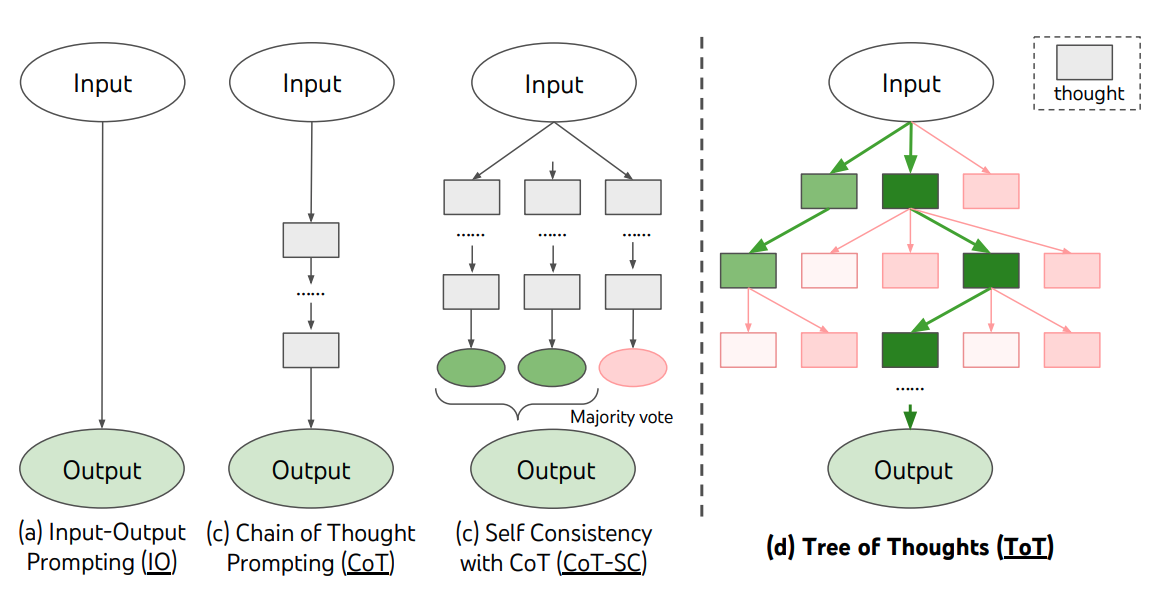
\includegraphics[width=0.8\textwidth]{img/chain_of_thoughts.png}
  \caption{Schematic illustrating various approaches to problem solving with LLMs. Each rectangle box represents a thought, which is a coherent language sequence that serves as an intermediate step toward problem solving.~\cite{yao2023tree}}\label{fig:chain_of_thoughts}
\end{figure}
\end{frame}

%-------------------------------
\section{Methodology}
\begin{frame}[allowframebreaks]
\frametitle{Problem definition}
\begin{itemize}
  \item Generating code has consistently posed a significant challenge with numerous applications, including creating code from natural languages, programming based on examples, and translating code. Nonetheless, for numerous programming tasks, \textbf{producing accurate code in a single try can be difficult}.~\cite{chen2023teaching}
  \item As per a study, average developers are expected to see a moderate increase in productivity, with the \textbf{overall productivity gain projected to be 32\% with the support of LLMs}.~\cite{eloundou2023gpts}
\end{itemize}
\end{frame}

\begin{frame}[allowframebreaks]
\frametitle{Approach}
\end{frame}

\begin{frame}[allowframebreaks]
\frametitle{Autonomous debugger}
\end{frame}

\begin{frame}[allowframebreaks]
\frametitle{Dataset}
\begin{itemize}
  \item MBPP \href{https://huggingface.co/datasets/mbpp}{Mostly Basic Python Programming}. The benchmark consists of around 1,000 crowd-sourced Python programming problems, designed to be solvable by entry-level programmers.~\cite{austin2021program}
  \item GHRB:~\href{https://github.com/coinse/GHRB}{GitHub Recent Bugs}~\cite{lee2023github}
  \item The MBPP dataset, renowned for code generation tasks, and the GHRB dataset, used for code debugging tasks, are two key resources in this field.
  \item The team behind GHRB has developed a method to gather recent bugs from GitHub, ensuring that this data has not been previously used in training LLMs.~$\rightarrow$~\textbf{This research will use the provided method to create a data science related bugs dataset for evaluation.}
\end{itemize}
\end{frame}

\begin{frame}[allowframebreaks]
\frametitle{Application}
This research will develop a plugin based on the open-sourced \href{https://github.com/jupyterlab/jupyter-ai?tab=readme-ov-file}{Jupyter AI} to assist data scientists in debugging their code.
\begin{figure}
  \centering
  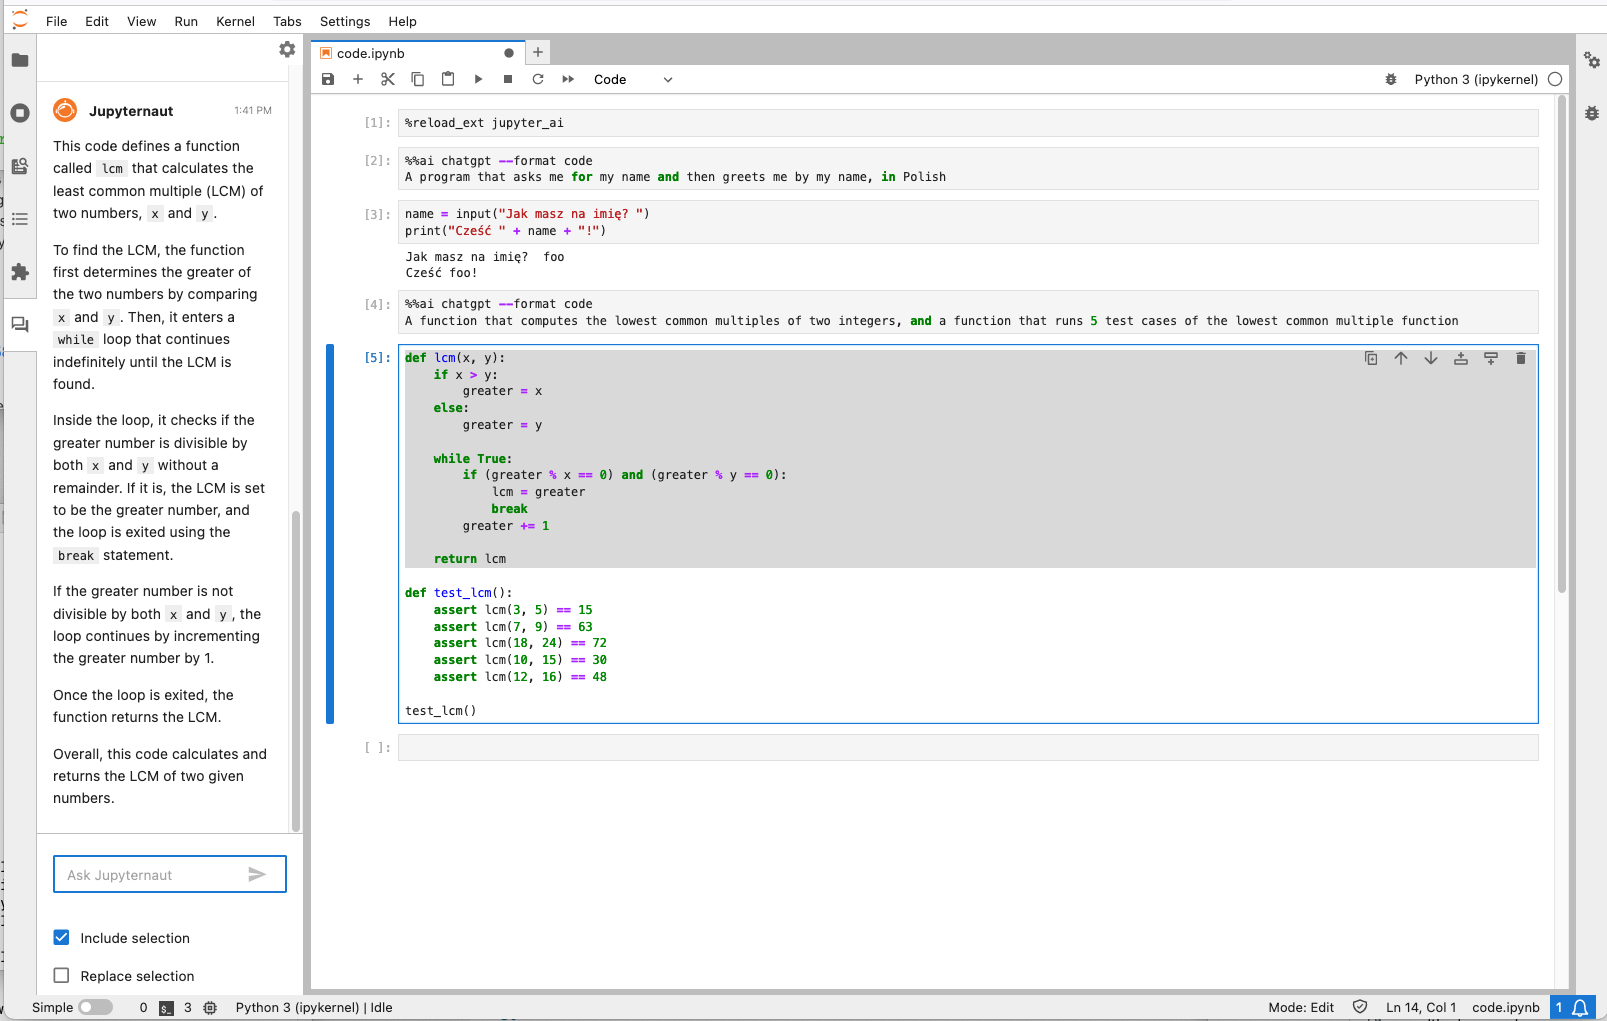
\includegraphics[width=0.6\textwidth]{img/jupyter_ai_screenshot.png}
  \caption{Jupyter AI connects generative AI with Jupyter notebooks.}\label{fig:jupyter_ai_screenshot}
\end{figure}
\end{frame}

\begin{frame}[allowframebreaks]
  \frametitle{Timeline}
  This research will develop a plugin based on the open-sourced \href{https://github.com/jupyterlab/jupyter-ai?tab=readme-ov-file}{Jupyter AI} to assist data scientists in debugging their code.
  \begin{figure}
    \centering
    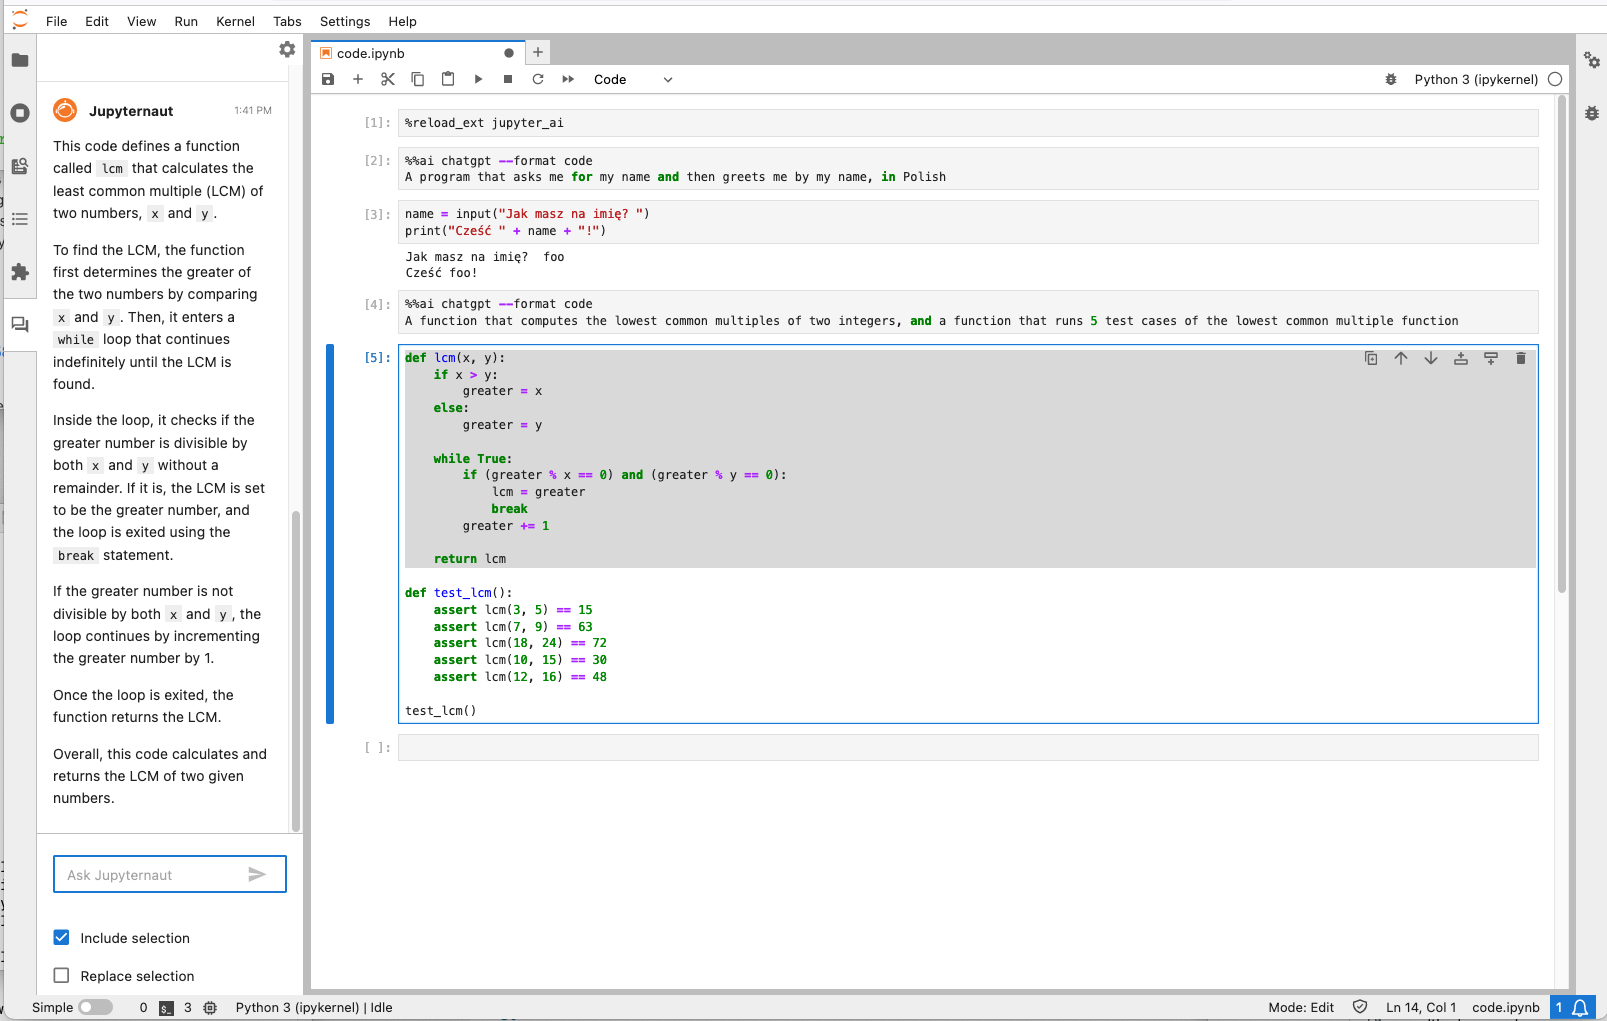
\includegraphics[width=0.6\textwidth]{img/jupyter_ai_screenshot.png}
    \caption{Jupyter AI connects generative AI with Jupyter notebooks.}\label{fig:jupyter_ai_screenshot}
  \end{figure}
  \end{frame}

%-------------------------------
\section{References}
\begin{frame}[allowframebreaks]
\frametitle{References}\scriptsize
\bibliography{references}
\bibliographystyle{plain}
\end{frame}

%-------------------------------
\begin{frame}
\Huge{\centerline{Thank You}}
\end{frame}

%-------------------------------
\section{Appendix}
\begin{frame}{Appendix}
\end{frame}
\end{document}
